%%%%%%%%%%%%%%%%%%%%%%%%%%%%%%%%%%%%%%%%%%%%%%%%%%%%%%%%%%%%%%%%%%%%%%%%%%%%%
% Chapter 1: Introducción 
%%%%%%%%%%%%%%%%%%%%%%%%%%%%%%%%%%%%%%%%%%%%%%%%%%%%%%%%%%%%%%%%%%%%%%%%%%%%%%%

%---------------------------------------------------------------------------------
\section{Introducción}
\label{1:sec:1}

\begin{itemize}
  \item Item 1 \cite{Bay1}
  \item Item 2
  \item Item 3
  \item Item 4
\end{itemize}

%---------------------------------------------------------------------------------
\section{Antecedentes y estado actual}
\label{1:sec:2}

Para explicar los antecedentes y el estado actual del tema en este proyecto se tendrán en cuenta las referencias citadas a continuación:

\begin{itemize}
  \item En un artículo publicado en 2017 \textit{"Teacher Configurable Coding Challenges for Block Languages"} se explica como una herramienta llamada \textbf{COPPER}\cite{Tumlin:2017:TCC:3017680.3022467}, una herramienta desarrollada para crear puzzles de código en una cuadrícula usando lenguajes de programación basado en bloques, similar a los realizados en la plataforma Code.org "Hour of Code", que tiene el potencial de incrementar el interés y el compromiso con el pensamiento computacional.
  \item En 2015, en la revista llamada \textbf{"ACM INROADS"}, publicó un artículo\cite{Wilson:2015:HCB:2786608.2746406} mencionando la ayuda recibida por la NSF (National Science Foundation), una agencia federal independiente creada por el Congreso de los Estados Unidos en 1950 para promover el progreso de la ciencia, la salud nacional y muchos otros aspectos relevantes para el país, con lo que muchos de los alumnos en colegios sin recursos o estudiantes de color tuvieran acceso a una educación, tanto secundaria como primaria, digna en las Ciencias de la Computación.
  \item Por último, en un artículo\cite{Brown:2016:PFD:2839509.2844661} publicado en 2016, en el libro llamado "Proceedings of the 47th ACM Technical Symposium on Computer Science Education"  se constata que las enseñanzas sobre la Ciencia de la Computación que se componen de actividades que usen la programación basada en bloques, como pueden ser con Scratch, Alice y las "Hour of Code" de Code.org, incentivan tanto a alumnos como profesores a indagar con más profundidad en el mundo del pensamiento computacional.

\end{itemize}

Cabe mencionar que uno de los recursos que usaremos para este proyecto sería su repositorio alojado en la plataforma \textbf{Github}, que supondría una ayuda a la hora de analizar el diseño de la página Code.org, de tal manera que podamos aportar unas estadísticas más concretas de cada alumno.

%---------------------------------------------------------------------------------
\section{Sección Tres}
\label{1:sec:3}

Bla, bla, bla  \ref{1:sec:1}

%---------------------------------------------------------------------------------
\section{Sección Cuatro}
\label{1:sec:4}

Bla, bla, bla

%------------------------------------------------------------------------------
\begin{figure}[!th]
\begin{center}
\includegraphics[width=0.5\textwidth]{images/arbolbinario.eps}
\caption{Ejemplo}
\label{fig:ArbolBinario}
\end{center}
\end{figure}
%------------------------------------------------------------------------------

